\documentclass[nocrop]{sesamanuel}
\usepackage{sesamanuelTIKZ}
\let\ifluatex\relax
\usepackage{hyperref}


%complement
\usepackage{tikz}  %   appel  général
\usepackage{pgf}  %   appel  général
\usepackage{tkz-tab}  %   extention  pour  les  tableaux  de  variations
\usetikzlibrary{arrows}  %   librairie  pour  les  flèches
\usetikzlibrary{patterns}  %   librairie  pour  les  hachures  et  les  pointillés

%theme perso
\NewThema{A}{a}{algèbre}{Algèbre}{ALGÈBRE}{PartieFonction}{A4}

\themaA
\begin{document}
\chapter{Les fonctions}
\cours
\section{Notion de fonction}
\begin{definition}
On appelle fonction toute correspondance définie d'un ensemble A appelé ensemble de départ vers un ensemble B appelé ensemble d'arrivé tel qu'à un élément de l'ensemble A, on associe un unique élément de l'ensemble B.
\end{definition}

\begin{exemple*1}

\end{exemple*1}

\section{Applications affines}
\begin{definition}
On appelle \emph{application affine}, toute application de la forme \emph{$f(x)=ax+b$}.
%\vspace{0.5cm}
\begin{exemple*1}
$f(x)=2x+3$ \quad ; \quad $g(x)=-3x+7$ \quad ; \quad $g(x)=-\frac{2}{3}x-\sqrt{3}$ sont des applications affines.
\end{exemple*1}
\end{definition}

\section{Image et antécédent par une application affine}

\section{Représentation graphique d'une application affine}

\section{Sens de variation d'une application affine}

\section{Applications linéaires}
\begin{definition}
On considère une droite $(D)$ et un point A n'appartenant pas à la droite $(D)$.\\
\begin{itemize}
\item On appelle \emph{projection orthogonale} du point A sur la droite $(D)$, la perpendiculaire à $(D)$ passant par A.
\item Si H est le point d'intersection de (D) et de la projection orthogonale de A sur $(D)$, alors le point H est appelé, le \emph{projeté orthogonal} du point A sur la droite $(D)$.
\end{itemize}
\end{definition}

\begin{definition}
La distance du point A à la droite (D) est la distance du point A et du projeté orthogonal de A sur $(D)$
\end{definition}



\exercicesbase
\begin{colonne*exercice}
\begin{exercice}[J'ai gagné!!!]
Un jeu consiste à tirer des boules de deux sacs différents A et B. Le sacs A contient des boules numérotées de 1 à 10. Le candidat choisi une boule du sac A, note son numéro puis effectue les calculs suivants:
\begin{itemize}
\item calculer le carré du numéro obtenu.
\item augmenté le résultat de 1.
\end{itemize}

Il retient le résultat puis tire une boule du sac B.
Le jeu est gagné si la boule tirer porte le résultat précédemment obtenu.
\begin{enumerate}
\item Trouve pour chaque boule du sac A, la boule du sac B qu'il faut pour gagner à ce jeu.
\item Si on désigne pour x le numéro de la boule du sac A, quel sera le numéro de la boule du sac B permettant de gagner?
\item Écris la fonction qui à tout numéro de la boule tirer du sac A, associe le numéro de la boule du sac B permettant de gagner au jeu.
\end{enumerate}
\end{exercice}

\begin{exercice}[calcul mental]
Soient $f$ et $g$ les fonctions qui s'expriment par $f(x)=x-9$ et $g(x)=-5x$. Calculer les expressions:
\begin{multicols}{3}
\begin{enumerate}
\item f(15)
\item f(-2)
\item f(5,5)
\item g(7)
\item g(-6)
\item g(0)
\end{enumerate}
\end{multicols}

\end{exercice}

\begin{exercice}
Soit la fonction qui, à tout nombre x, associe le nombre $x^2-3$.
\begin{enumerate}
\item Recopie et complète: $f: x \mapsto \ldots$ et $f(x)=\ldots$
\item Trois élèves d'une classe de $3^{eme}$ affirment:
\begin{itemize}
\item Vianney:
Au nombre 4 on associe 13 par la fonction $f$.
\item Stéphanie:
$f(5)$ est égal à 22 et $f(-5)$ aussi! 
\item Josiane:
On peut également écrire: $f: 7 \mapsto 46$ et $f: 0 \mapsto -3$
\end{itemize}
\end{enumerate}
\end{exercice}

\begin{exercice}
Traduis chacune des informations suivantes par une égalité:
\begin{enumerate}
\item L'image de 5 par la fonction $f$ est 4.
\item 8 est l'image de -3 par la fonction $g$.
\item 0 a pour image 2 par la fonction $f$.
\end{enumerate}
\end{exercice}

\begin{exercice}
Traduis chacune des informations suivantes par une égalité:
\begin{enumerate}
\item $f$ est la fonction qui, à chaque durée $t$ d'un trajet, associe la distance $d$ parcourue.
\item 4 est un antécédent de 9 par la fonction f.
\item 0 a pour antécédent 7 par la fonction $f$.
\item Les antécédents de 3 par la fonction f sont -1 et 3.
\end{enumerate}
\end{exercice}

\begin{exercice}
On considère le tableau de valeurs suivant:\\
\begin{tabular}{|c|c|c|c|c|c|c|c|}
\hline 
x & -3 & -2 & -1 & 0 & 1 & 2 & 3 \\ 
\hline 
$f(x)$ & 7 & 2 & -1 & -2 & -1 & 2 & 7 \\ 
\hline 
\end{tabular} 
\begin{enumerate}
\item D'après ce tableau : 
\begin{enumerate}
\item quelle l'image 0 par la fonction $f$?
\item quels sont les antécédents par $f$ du nombre 2?
\end{enumerate} 
\item Dans un repère orthonormé place les points de coordonnées $(x;f(x))$.
\item Relie les points obtenus par une courbe.
\end{enumerate}
\end{exercice}

\begin{exercice}
Le graphique ci-dessous représente une fonction k pour x compris entre 0 et 16.
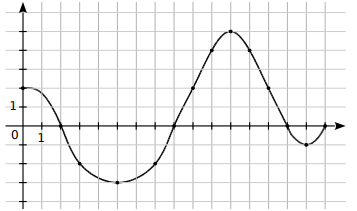
\includegraphics[scale=0.7]{images/fonction_img1.png}\\
\begin{enumerate}
\item L'image de 5 par la fonction k est \ldots
\item L'image de 8 par la fonction k est \ldots
\item Quels sont les antécédents de 2 par k ?
\item Quels nombres ont pour image − 2 par k ?
\item Quels sont les antécédents de 0 par k ?
\item $f(5)=\ldots$.
\end{enumerate}
\end{exercice}

\begin{exercice}
Ce graphique représente une fonction g.
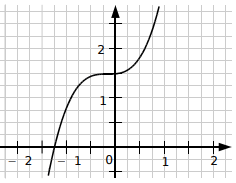
\includegraphics[scale=0.8]{images/fonction_img2.png} \\
Reproduis puis complète le tableau de valeurs suivants:\\
\begin{tabular}{|c|c|c|c|c|}
\hline 
x & -1,25 & • & -1 & • \\ 
\hline 
$g(x)$ & • & 1,5 & • & 1,25 \\ 
\hline 
\end{tabular} 
\end{exercice}

\begin{exercice}
On donne la fonction f definie par\\ $f(x)=x^2-3x-8$ et on nomme $(\mathcal{C}_f)$ sa courbe représentative.\\Parmi les points suivants, quels sont ceux qui appartiennent à $(\mathcal{C}_f)$: $A(0;-8)$ ;$B(1;7)$ ; $C(-2;2)$?
\end{exercice}

\end{colonne*exercice}


\exercicesappr


\connaissances
\begin{acquis}
\begin{itemize}
\item  Premier  point  à  connaître.
\item  Autre  point  à  savoir  faire.
\item  Dernier  point  devant  être  su.
\end{itemize}
\end{acquis}
\QCMautoevaluation{texte  introductif}
\begin{QCM}
\begin{EnonceCommunQCM}
Pour  les  questions  \RefQCM{premier-qcm}  à
\RefQCM{deuxieme-qcm},  $f$  désigne  une fonction  affine.
\end{EnonceCommunQCM}
\begin{GroupeQCM}
\begin{exercice}\label{premier-qcm} La  courbe  de  $f$  est
\begin{ChoixQCM}{3}
\item  une  droite
\item  une  parabole
\item  autre
\end{ChoixQCM}
\end{exercice}
\begin{corrige}
\reponseQCM{a}
\end{corrige}
\begin{exercice}\label{deuxieme-qcm}
$f(3)$
\begin{ChoixQCM}{3}
\item  vaut  la  moitié  de  $f(6)$
\item  vaut  le  double  de  $f(6)$
\item  on  ne  peut  pas savoir
\end{ChoixQCM}
\end{exercice}
\begin{corrige}
\reponseQCM{c}
\end{corrige}
\end{GroupeQCM}
\end{QCM}

\chapter{Les équations dans $\mathbb{R} \times \mathbb{R}$}

\chapter{Les inéquations dans $\mathbb{R} \times \mathbb{R}$}

\chapter{Statistiques}

\end{document}
